\newpage
\section{Resultados}

\subsection{Modulação PSK}

	A princípio foi realizada a montagem e conexão dos equipamentos de acordo com a Figura \ref{fig:montagem}(a), conforme mostram as Figuras \ref{fig:6} e \ref{fig:7}.

	\begin{figure}[H]
		\centering
	  	\caption{Montagem do transmissor PSK.}
	   	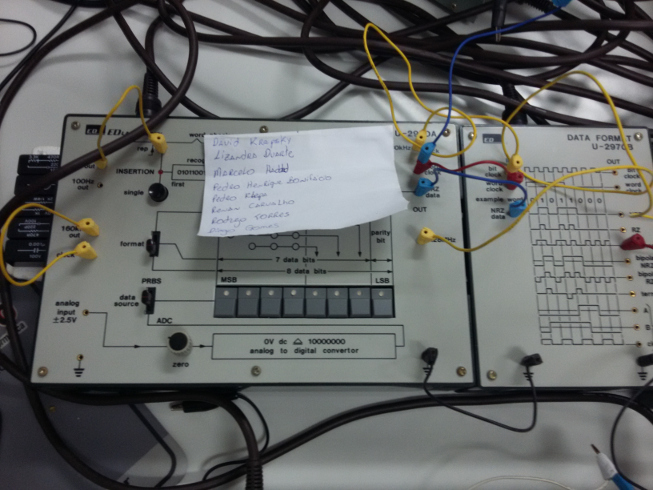
\includegraphics[scale=0.5]{6}
   	
	   	\small Fonte: Autoria própria.
	   	\label{fig:6}
	\end{figure}

	\begin{figure}[H]
	 	\centering
	 	\caption{Montagem do transmissor PSK (continuação).}
	 	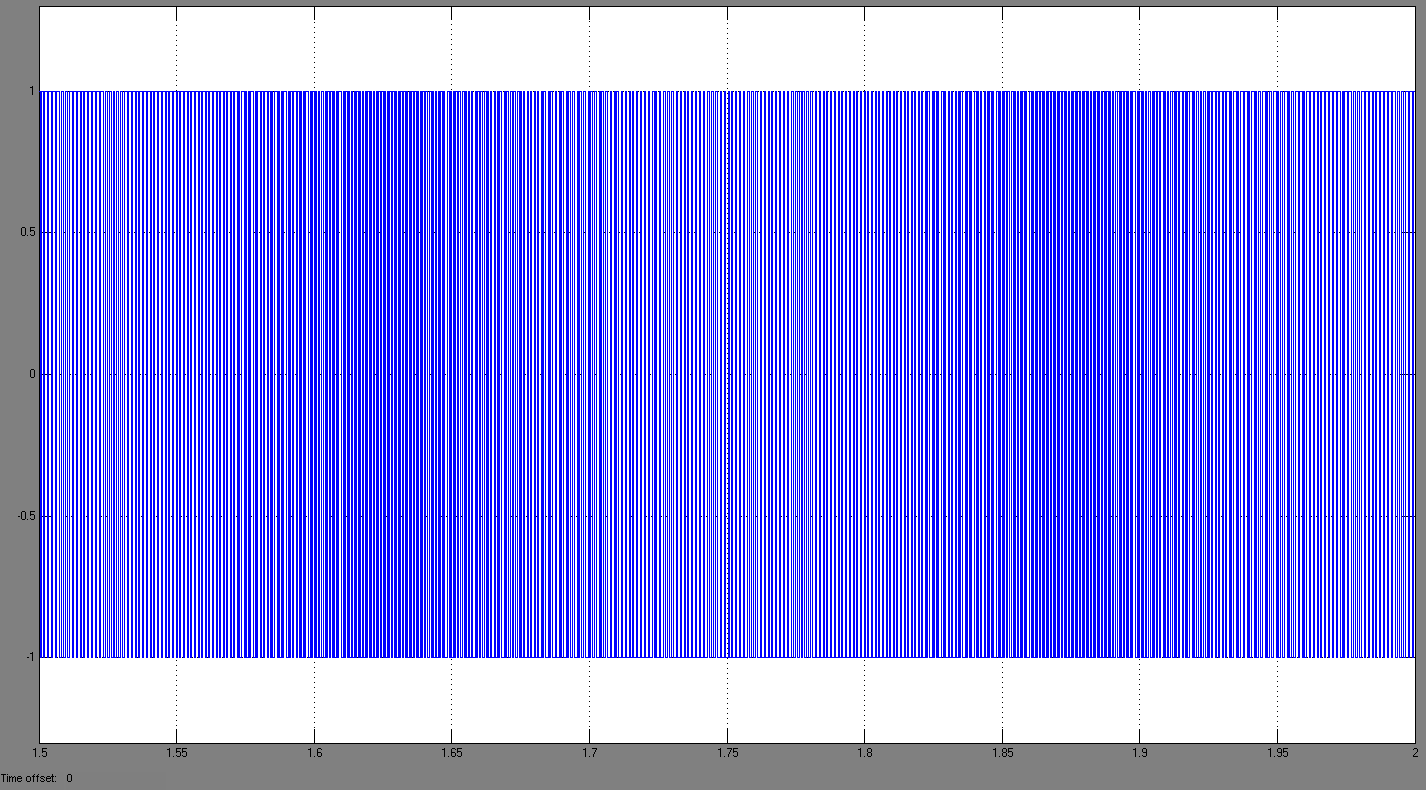
\includegraphics[scale=0.5]{7}
 	
	 	\small Fonte: Autoria própria.
	 	\label{fig:7}
	\end{figure}
	
	Em seguida, foi observado o nível DC do sinal bi-fase, onde foi obtido um valor de $2,22V_{RMS}$, conforme mostra a Figura \ref{fig:1}.
	
	\begin{figure}[H]
		\centering
		\caption{Nível DC do sinal bi-fase.}
		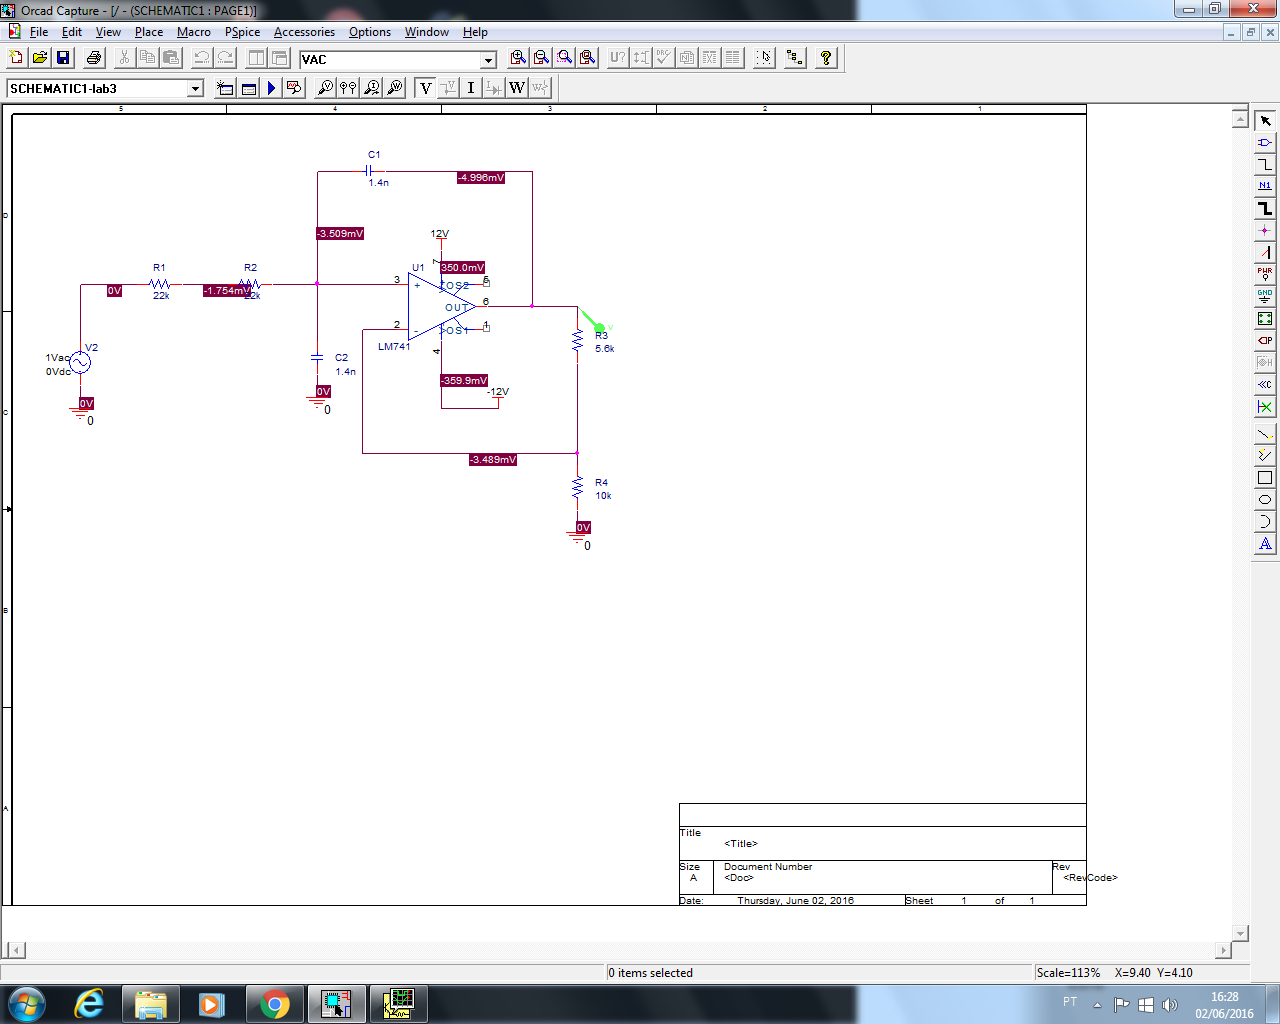
\includegraphics[scale=0.3]{1}
		
		\small Fonte: Autoria própria.
		\label{fig:1}
	\end{figure}
	
	Foi ajustado o controle de ganho e fase, de modo a obter duas ondas, nas ligações 10 e 12, com amplitude aproximada e deslocamento de fase de aproximadamente $90º$, visto na figura \ref{fig:2}.

	\begin{figure}[H]
		\centering
		\caption{Sinais nas ligações 10 e 12.}
		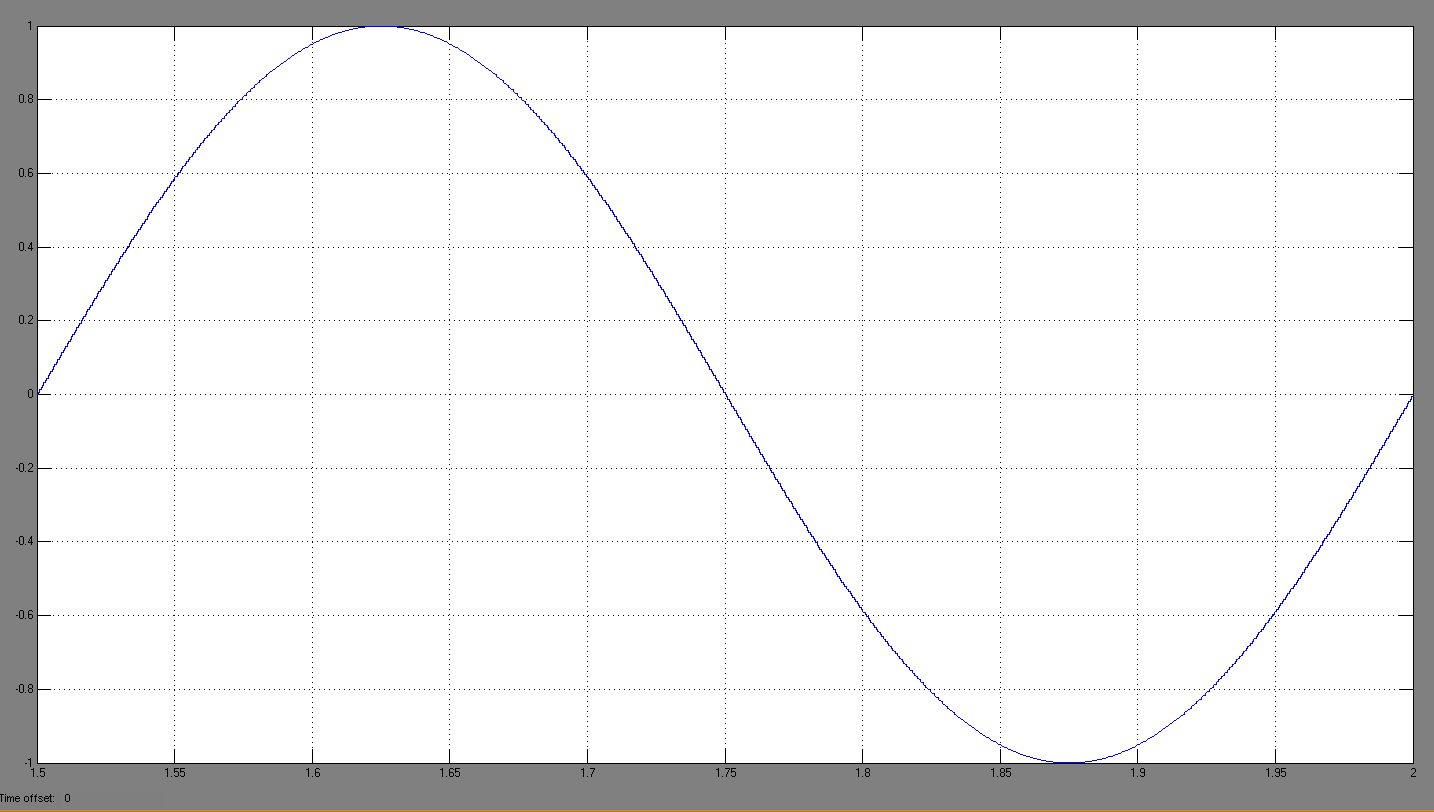
\includegraphics[scale=0.3]{2}
		
		\small Fonte: Autoria própria.
		\label{fig:2}
	\end{figure}	
	
	Em seguida, a constante DC do modulador inferior foi ajustada de modo a obter uma tensão positiva de $2V$, apresentado na Figura \ref{fig:12}. Note na fique que o eixo vertical do canal 2 está deslocado, conforme a indicação $2\blacktriangleright$ no canto esquerdo da tela.
	
	\begin{figure}[H]
		\centering
		\caption{Constante DC do modulador inferior.}
		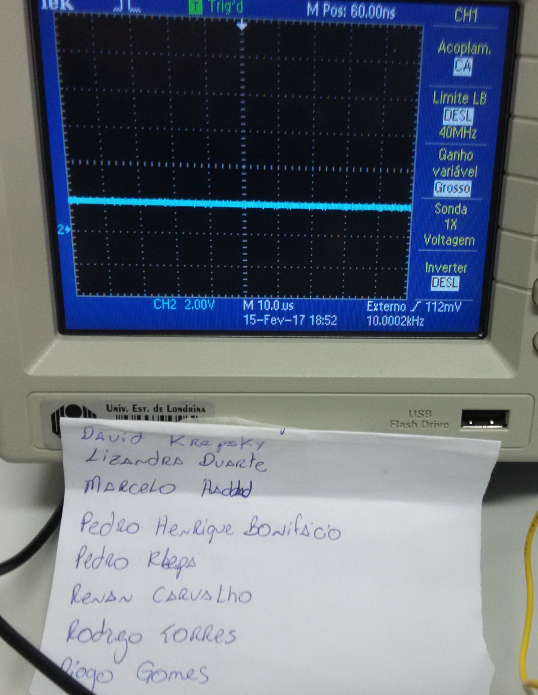
\includegraphics[scale=0.3]{12}
		
		\small Fonte: Autoria própria.
		\label{fig:12}
	\end{figure}
	
	O sinal modulado em fase obtido na ligação 14 é mostrado na Figura \ref{fig:14} (canal 2 do osciloscópio), junto com a portadora (canal 1 do osciloscópio).
	
	\begin{figure}[H]
		\centering
		\caption{Sinal modulado em fase.}
		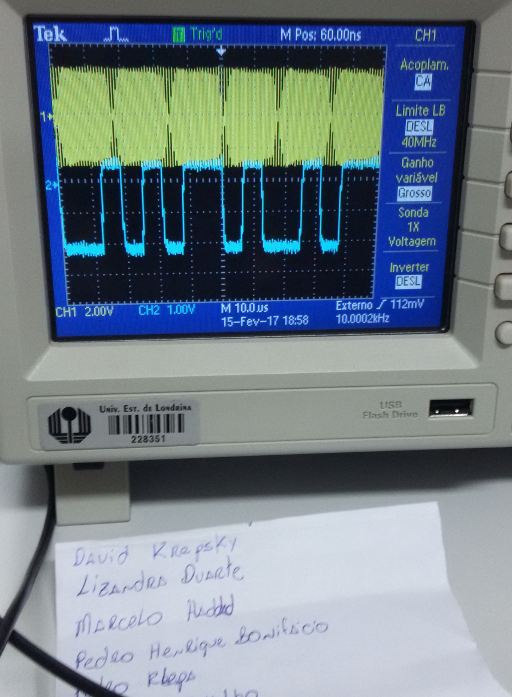
\includegraphics[scale=0.3]{14}
		
		\small Fonte: Autoria própria.
		\label{fig:14}
	\end{figure}
	
	Na Figura \ref{fig:13}, pode observar o efeito da limitação de banda na forma de onda da saída, onde o sinal sofre um deslocamento em fase e amplitude.

	\begin{figure}[H]
		\centering
		\caption{Efeito da limitação da largura de banda na forma de onda da saída.}
		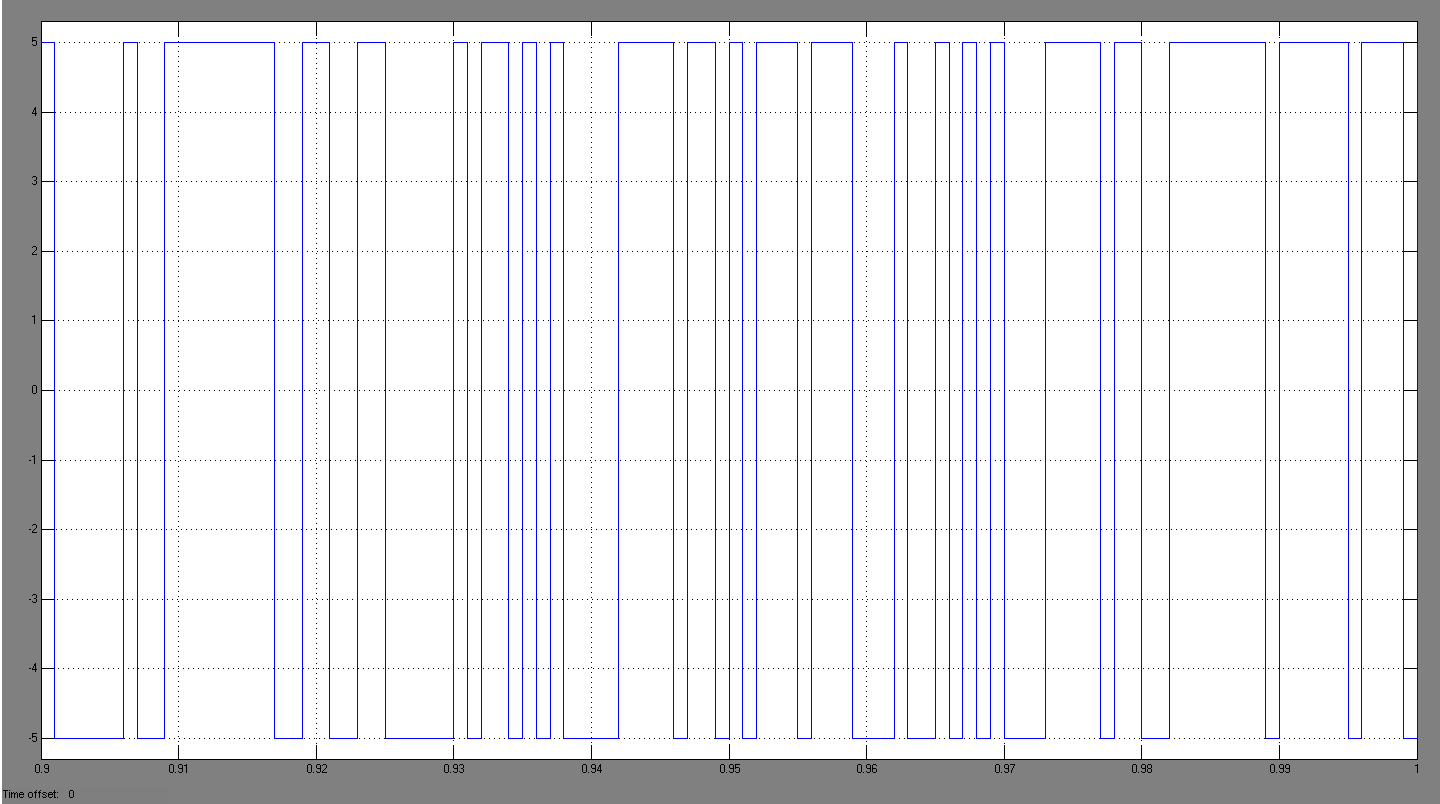
\includegraphics[scale=0.3]{13}
		
		\small Fonte: Autoria própria.
		\label{fig:13}
	\end{figure}	
	
\subsection{Demodulação PSK}

	A montagem e conexão dos equipamento para demodulação do sinal PSK se deu conforme as Figuras \ref{fig:8}, \ref{fig:9} e \ref{fig:10}.
	
	\begin{figure}[H]
		\centering
		\caption{Montagem do demodulador PSK.}
		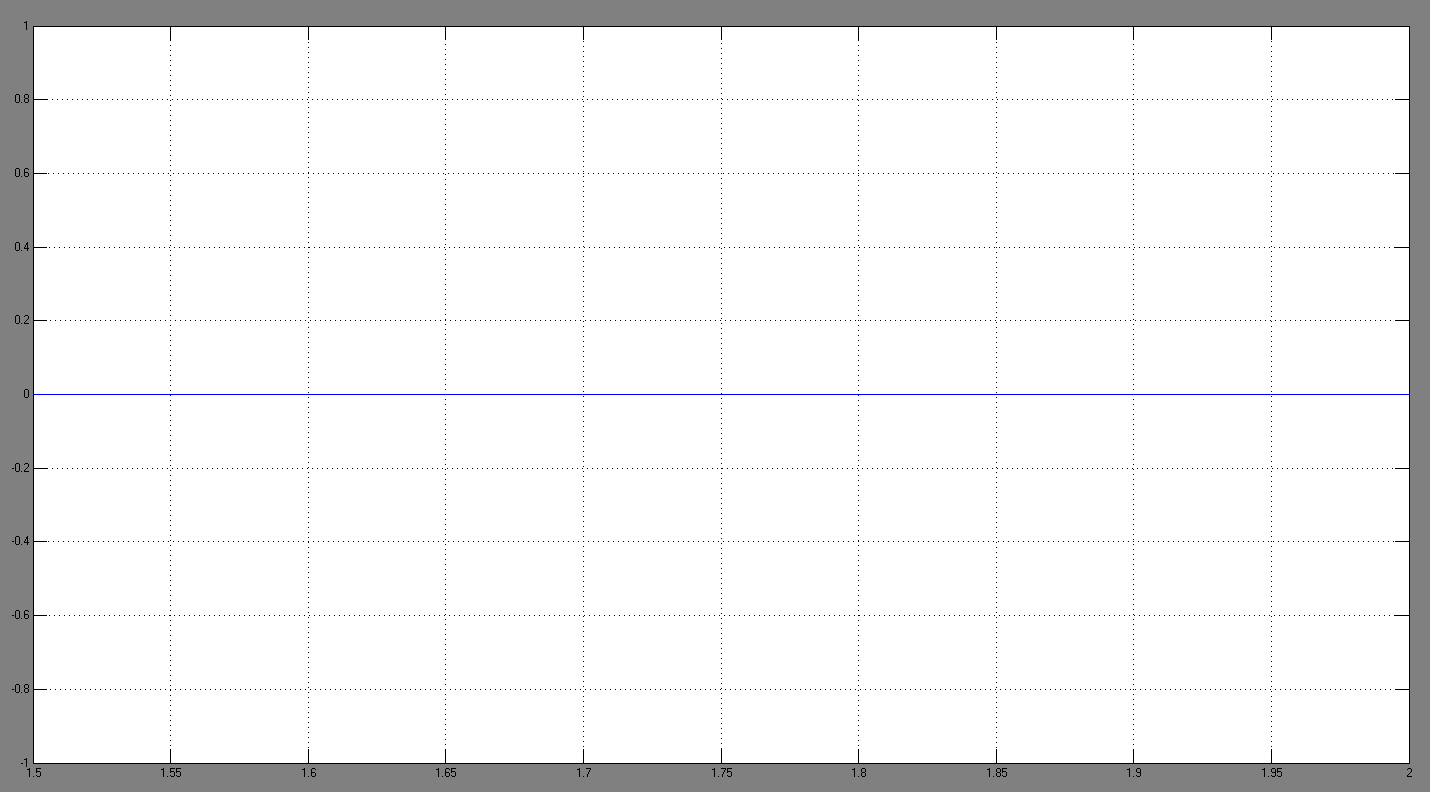
\includegraphics[scale=0.5]{8}
		
		\small Fonte: Autoria própria.
		\label{fig:8}
	\end{figure}
	
	\begin{figure}[H]
		\centering
		\caption{Montagem do demodulador PSK.}
		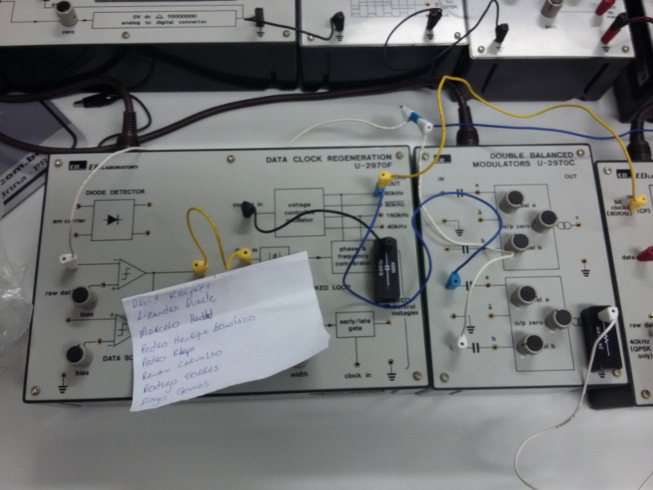
\includegraphics[scale=0.5]{9}
		
		\small Fonte: Autoria própria.
		\label{fig:9}
	\end{figure}
	
	\begin{figure}[H]
		\centering
		\caption{Montagem do demodulador PSK.}
		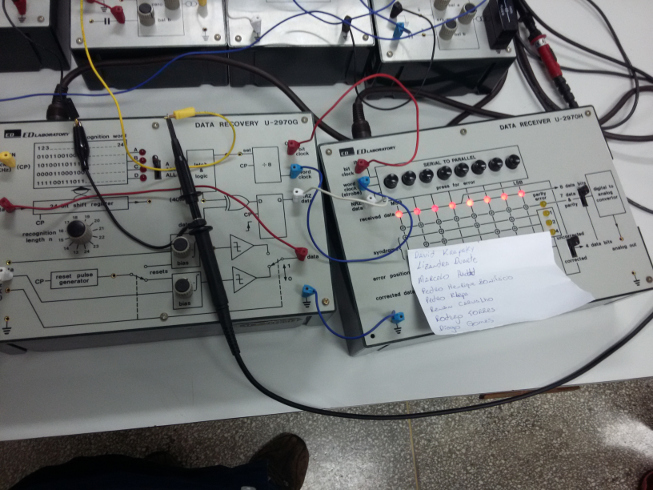
\includegraphics[scale=0.5]{10}
		
		\small Fonte: Autoria própria.
		\label{fig:10}
	\end{figure}

	A Figura 15 mostra a portadora recuperada no CH1 do osciloscópio.
	
	\begin{figure}[H]
		\centering
		\caption{Portadora recuperada no CH1.}
		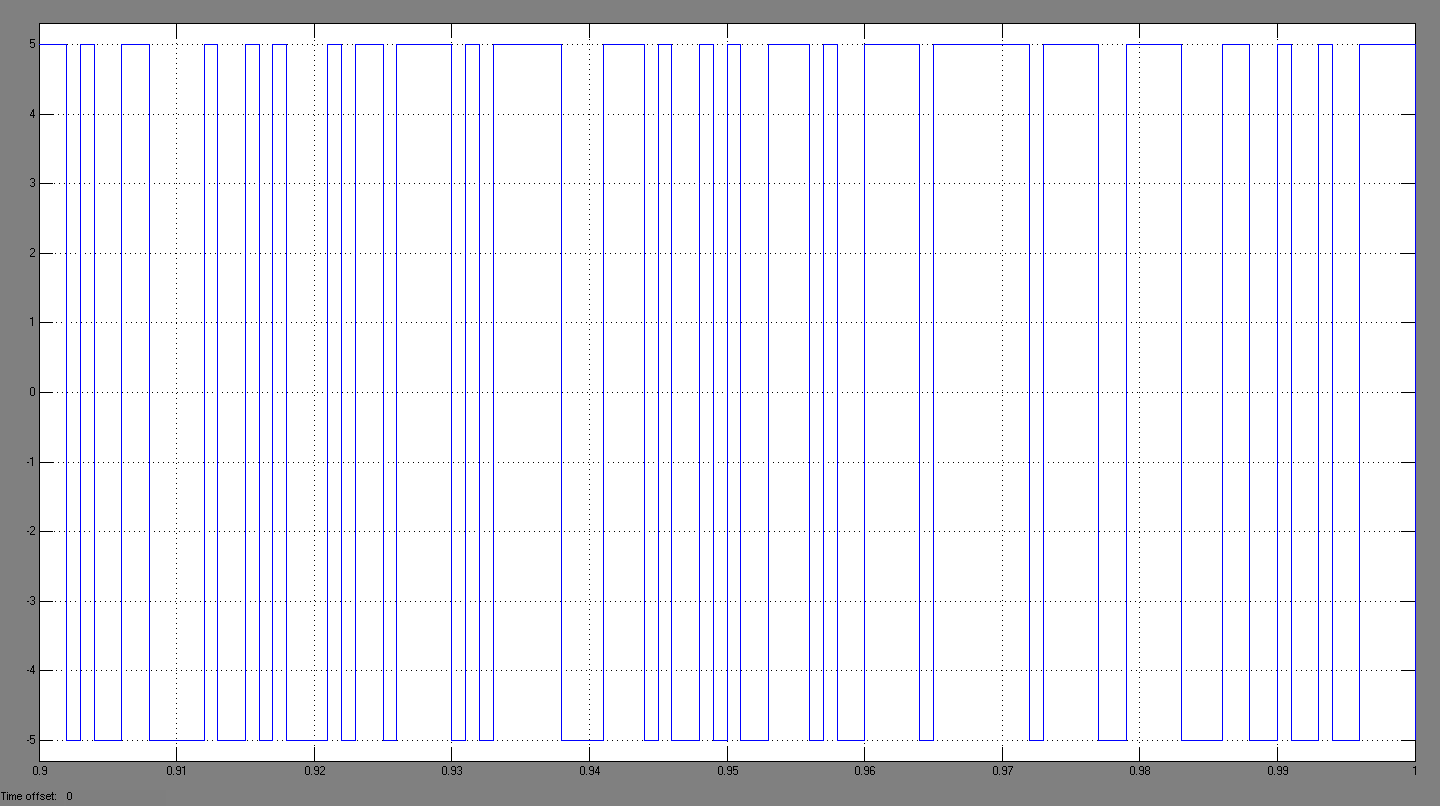
\includegraphics[scale=0.3]{15}
		
		\small Fonte: Autoria própria.
		\label{fig:15}
	\end{figure}
	
	A Figura \ref{fig:16} mostra os dados enviados (00110100) e a Figura \ref{fig:17} mostra o sinal bi-fase enviado (ligação 9) e sinal dos dados recuperados (ligação 20). Observe que existe o atraso de 1 bit, devido ao processo de integração do sinal recebido.
	
	\begin{figure}[H]
		\centering
		\caption{Palavra de dados enviada 00110100.}
		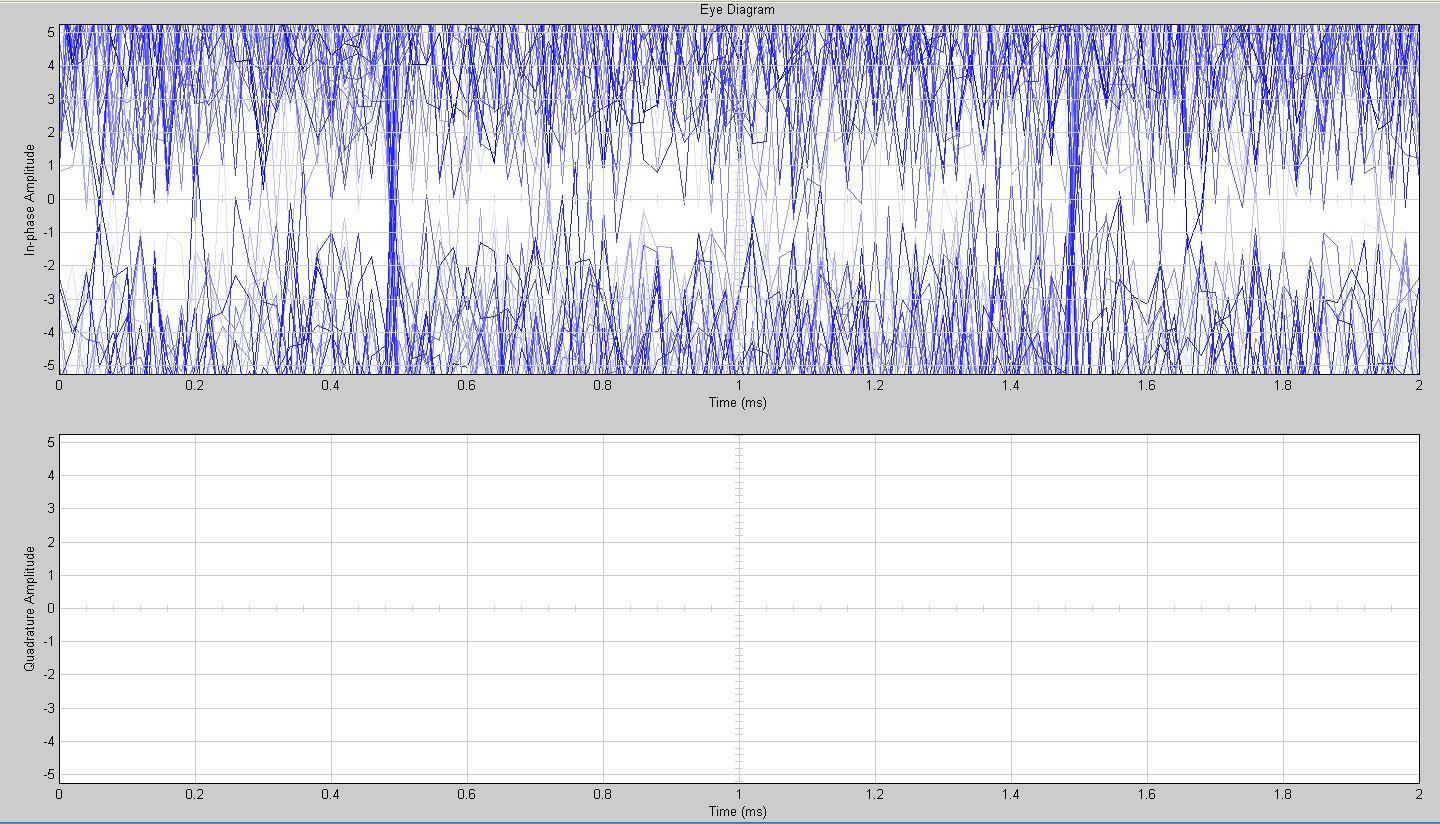
\includegraphics[scale=0.5]{16}
		
		\small Fonte: Autoria própria.
		\label{fig:16}
	\end{figure}
	
	\begin{figure}[H]
		\centering
		\caption{Sinal bi-fase enviado e recebido.}
		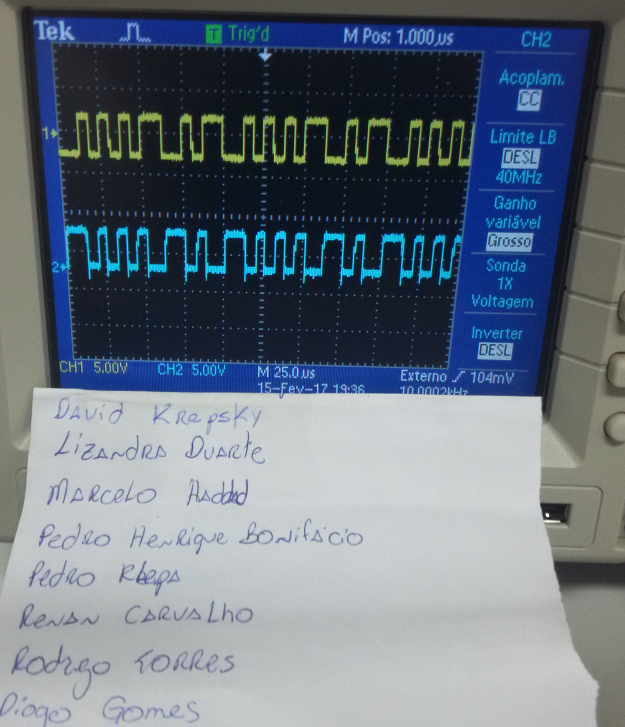
\includegraphics[scale=0.3]{17}
		
		\small Fonte: Autoria própria.
		\label{fig:17}
	\end{figure}
	
	Por último, removendo a ligação 1 e alterando o controle da fase para mais que $90º$, com os dados todos em 1, foi observado que os dados de saída ficam invertido, isto é, em vez da saída ser 00000000, a obtida foi 111111, como pode ser observado na Figura \ref{fig:24} e Figura \ref{fig:23}.
	
	\begin{figure}[H]
		\centering
		\caption{Sequência enviada 00000000 com deslocamento de fase maior que $90º$.}
		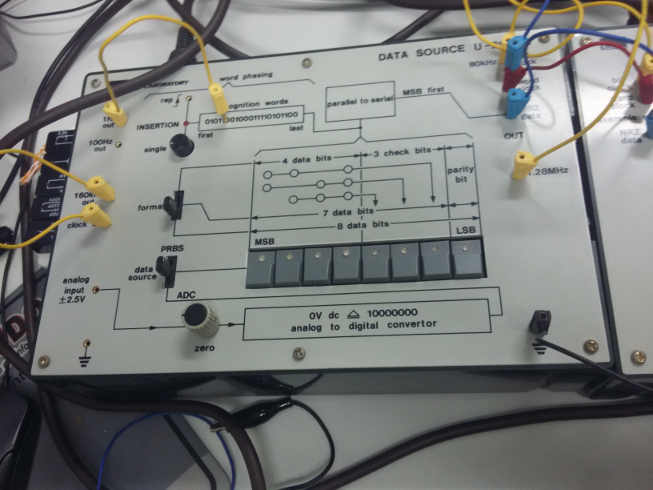
\includegraphics[scale=0.5]{24}
		
		\small Fonte: Autoria própria.
		\label{fig:24}
	\end{figure}
	
	\begin{figure}[H]
		\centering
		\caption{Dados recuperados 11111111 com deslocamento de fase maior que $90º$.}
		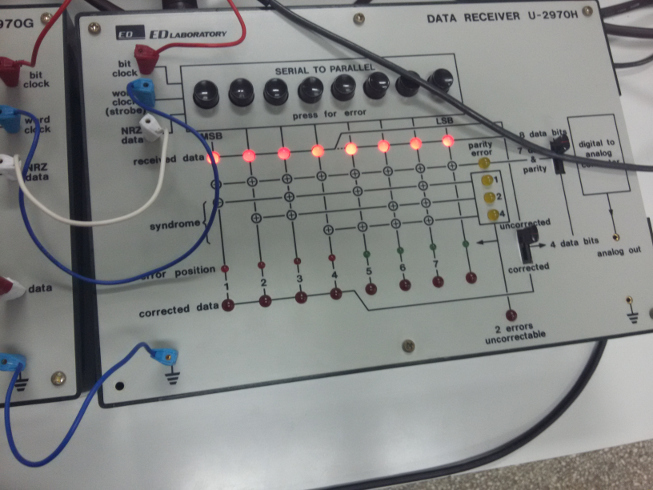
\includegraphics[scale=0.5]{23}
		
		\small Fonte: Autoria própria.
		\label{fig:23}
	\end{figure}